\chapter{Vorbereitung}

\section{Technische Grundlagen}

Zur Untersuchung optischer Phänomene müssen umfangreiche experimentelle Aufbauten
mit komplizierten Geräten verwendet werden. Hier soll kurz in die für diesen
Versuch notwendige Technik eingeführt werden.


    \subsection{Halbleiter}

Den Halbleiter zeichnet eine Bandlücke zwischen \emph{Valenzband} und 
\emph{Leitungsband} aus, das kleiner ist als beim Isolator, aber groß genug,
um sich vom Leiter abzugrenzen. In der Technik findet sich der Halbleiter inzwischen
überall. Auch in diesem Experiment wird der Halbleiter Verwendung finden.
\begin{figure}
  \centering
  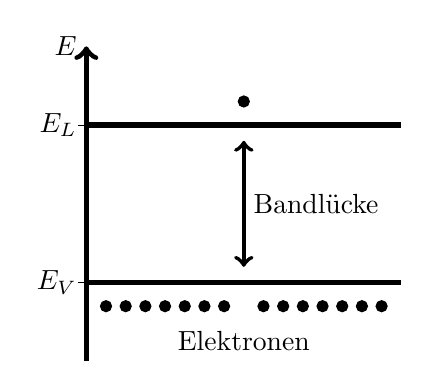
\begin{tikzpicture}
%Achse 
	\draw[draw=black,line width=2pt,->] (0,0) -- (0,4);
	\draw (-0.1,1) -- (0.1,1);
	\draw (-0.1,3) -- (0.1,3);
%Beschriftung
	\draw (0,1) node 
	  [anchor=east]
	  {$E_V$};
  \draw (0,3) node 
	  [anchor=east]
	  {$E_L$};
	\draw (0,4) node
		[anchor=east]
		{$E$};
%Bänder
	\draw[draw=black,line width=2pt] (0,1) -- (4,1);
  \draw[draw=black,line width=2pt] (0,3) -- (4,3);
	%\draw (4,1) node
	%	[anchor=west]
	%	{Valenzband};
	%\draw (4,3) node
	%	[anchor=west]
	%	{Leitungsband};
%Elektronen im Band
  \foreach \x in {1,2,...,7,9,10,...,15}{
	  \filldraw (\x/4,0.7) circle (2pt);}
	\filldraw (2,3.3) circle (2pt);
	\draw (2,0.5) node
		[anchor=north]
		{Elektronen};
%Bandlücke
	\draw[line width=1.5pt,<->] (2,1.2) -- (2,2.8);
	\draw (2,2) node
	  [anchor=west]
		{Bandlücke};
\end{tikzpicture}


  \caption{Bandstruktur eines Halbleiters}
  \label{abb:band-halbleiter}
\end{figure}
In der Technik werden Halbleiter meist \emph{dotiert}. Hierbei werden gezielt 
Fremdatome in das Gitter eingebracht, um so das Verhältnis von Lochdichte zu
Elektronendichte zu manipulieren. \emph{Donatoren} geben Elektronen an das Gitter 
ab, während \emph{Akzeptoren} diese aufnehmen und so ein zusätzliches Loch 
schaffen. Da die Bindungsenergie des Donators kleiner als 
\begin{figure}
  \centering
  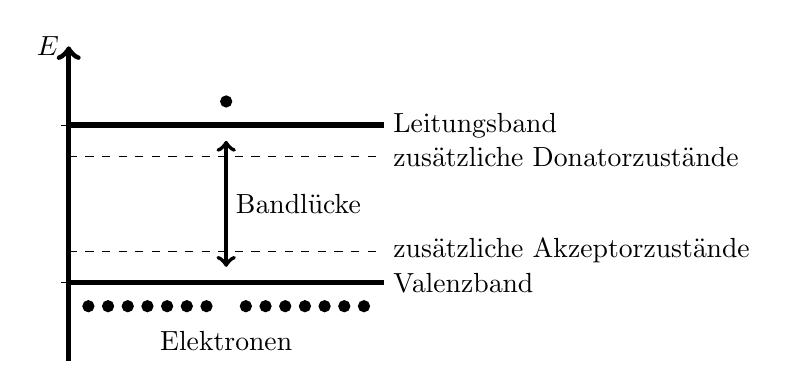
\begin{tikzpicture}
%Achse 
	\draw[draw=black,line width=2pt,->] (0,0) -- (0,4);
	\draw (-0.1,1) -- (0.1,1);
	\draw (-0.1,3) -- (0.1,3);
%Beschriftung
	%\draw (0,1) node 
	%  [anchor=east]
	%  {$E_V$};
  %\draw (0,3) node 
	%  [anchor=east]
	%  {$E_L$};
	\draw (0,4) node
		[anchor=east]
		{$E$};
%Bänder
	\draw[draw=black,line width=2pt] (0,1) -- (4,1);
  \draw[draw=black,line width=2pt] (0,3) -- (4,3);
	\draw (4,1) node
		[anchor=west]
		{Valenzband};
	\draw (4,3) node
		[anchor=west]
		{Leitungsband};
%Elektronen im Band
  \foreach \x in {1,2,...,7,9,10,...,15}{
	  \filldraw (\x/4,0.7) circle (2pt);}
	\filldraw (2,3.3) circle (2pt);
	\draw (2,0.5) node
		[anchor=north]
		{Elektronen};
%Bandlücke
	\draw[line width=1.5pt,<->] (2,1.2) -- (2,2.8);
	\draw (2,2) node
	  [anchor=west]
		{Bandlücke};
%Donator- und Akzeptorzustände
	\draw[dashed] (0,1.4) -- (4,1.4);
	\draw (4,1.4) node
		[anchor=west]
		{zusätzliche Akzeptorzustände};
	\draw[dashed] (0,2.6) -- (4,2.6); 
	\draw (4,2.6) node
		[anchor=west]
		{zusätzliche Donatorzustände};
\end{tikzpicture}

  \caption{Bandstruktur eines dotierten Halbleiters}
  \label{abb:band-dotiert}
\end{figure}


    \subsection{Laser}

Der Laser (\f light \f amplification by \f stimulated \f emission of \f radiation)
ist eine Lichtquelle, die sich durch hohe Strahlungsintensität, einen engen 
Frequenzbereich, starker Bündelung des Strahls und einer großen Kohärenzlänge 
auszeichnet.
\begin{figure}[h]
  \centering
    \import{Abb/}{emission.pdf_tex}
  \caption{Wechselwirkung zwischen Photonen und Elektronen im Atom}
  \label{abb:emission}
\end{figure}
Zur Lichterzeugung wird die \emph{spontane} und \emph{induzierte Emission} 
ausgenutzt, die in Abbildung \ref{abb:emission} skizziert ist. Ein Photon kann
ein gebundenes Elektron durch \emph{Absorption} auf ein höheres Energieniveau 
heben. Selbiges kann durch \emph{spontane Emission} unter Abgabe eines Photons
zurück in das niedrigere Niveau wechseln. Trifft dieses Photon auf ein weiteres
angeregtes Elektron, so kann dieses Elektron zur Emission angeregt werden, zur
\emph{induzierten Emission}. Wichtig ist hierbei, dass alle Photonen die gleiche
Energie tragen. Das Licht ist also monochromatisch. \par
Soll mithilfe dieses Prinzips ein intensiver Strahl erzeugt werden, so müssen 
möglichst viele Elektronen in diesen angeregten Zustand gebracht werden. Hierzu
verwendet man eine \emph{Pumpquelle}, siehe Abbildung \ref{abb:aufbau_laser}.
Diese Pumpe regt im \emph{aktiven Material},
also das Material, in dem die Emission stattfinden soll, die Elektronen an, sodass
mehr Elektronen im energetisch höheren Energieband aufhalten. Dieser Zustand wird
\emph{Besetzungsinversion} genannt. Durch spontane Emission wandern erste Photonen
durch das aktive Material und induzieren weitere Emission. 
Ein \emph{optischer Resonator}, oft verwirklicht durch zwei Spiegel, reflektiert nun
die Photonen immer wieder zurück in das aktive Material, wodurch sich eine stehende
Welle bildet. Der vordere Spiegel lässt immer einen Teil der Strahlung entweichen.
So entsteht ein homogener, intensiver Strahl. 
\begin{figure}[h]
  \centering
  \import{Abb/}{aufbau_laser.pdf_tex}
  \caption{Aufbau eines Lasers}
  \label{abb:aufbau_laser}
\end{figure}

Zur Versuchsdurchführung wird eine besondere Bauart des Lasers verwendet, der 
\emph{Faserlaser}. Dieser gibt statt einem kontinuierlichen Strahl kurze Pulse ab.
Der Aufbau ist hier komplexer, siehe Abbildung \ref{abb:faser}.
\begin{figure}[h]
  \centering
  \import{Abb/}{faserlaser.pdf_tex}
  \caption{Aufbau eines Faserlasers}
  \label{abb:faser}
\end{figure}
Das aktive Medium ist eine Erbium-dotierte Glasfaser. Durch eine Leuchtdiode, in der
Abbildung \emph{Pump Diode}, wird eine Besetzungsinversion der Erbium-Ionen
hergestellt. An den Enden der Faser bilden zwei teildurchlässige Spiegel den 
Resonator. Durch einen sättigbaren Absorber, \emph{SAM}, der nur kurze intensive
Impulse transmittiert, wird der gepulste Charakter des Lasers erreicht. Nach dem 
Verlassen des Oszillators erfolgt eine weitere Verstärkung in einer dotierten 
Glasfaser, wieder durch eine Diode gepumpt, bevor der Impuls ausgesendet wird. 
\autocite{phying, zinth}

    \subsection{Photodiode}


    \subsection{Lock-In Verstärker}


    \subsection{Pump-Probe Versuch}

\section{Nichtlineare Optik}
    \subsection{Doppelbrechung}

    \subsection{Phasenanpassung}

    \subsection{Nichtlineare Autokorrelation}

